% Model 1 sketch: logic chain, formulas, algorithm, results. Figures from Figures/M1 and Reports/M1.
\clearpage
\section{Model 1: Coupled Vegetation--Water--Sand Dynamics}\label{sec:model1}
Task~1 asks how cover and soil water on a desert-margin section evolve together, and what drives them. Our answer is a chain of four links:

\begin{center}
\begin{tikzpicture}[font=\normalsize,
  chainbox/.style={draw, rounded corners=2pt, line width=0.8pt, minimum width=1.6cm, minimum height=0.9cm},
  wat/.style={chainbox, draw=wfdy, fill=wfdy!8, text=wfdy},
  veg/.style={chainbox, draw=wfyr, fill=wfyr!8, text=wfyr},
  lk/.style={-{Stealth[length=6pt]}, line width=1pt},
  num/.style={circle, fill=white, draw, inner sep=0.5pt, font=\scriptsize\bfseries, minimum size=12pt}]
\definecolor{wfdy}{HTML}{2B6CB0}\definecolor{wfyr}{HTML}{18473C}
\node[wat] (a) {$P,\ I$};
\node[wat, right=1.5cm of a] (b) {$M_j$};
\node[wat, right=1.5cm of b] (c) {$\overline W_t$};
\node[veg, right=1.5cm of c] (d) {$V_t$};
\draw[lk, wfdy] (a) -- node[num, draw=wfdy, text=wfdy] {a} (b);
\draw[lk, wfdy] (b) -- node[num, draw=wfdy, text=wfdy] {b} (c);
\draw[lk, wfyr] (c) -- node[num, draw=wfyr, text=wfyr] {c} (d);
\draw[lk, wfyr] (d.south) -- ++(0,-0.5) -| (b.south);
\node[num, draw=wfyr, text=wfyr] at ($(c.south)+(0,-0.5)$) {d};
\end{tikzpicture}
\end{center}

\noindent \textcircled{\scriptsize a} Rain $P$ and irrigation $I$ fill a root-zone store $M_j$; \textcircled{\scriptsize b} the store decides the share $\overline W_t$ of the plants' water demand that is met; \textcircled{\scriptsize c} that share drives the change in cover $V_t$ through growth against decay and wind damage; \textcircled{\scriptsize d} cover in turn sets next year's demand on the store and how much wind reaches the ground, closing the loop. 

Figure~\ref{fig:m1-struct} adds the data behind each link. The reference section is the Yutian--Minfeng southern margin (Category~I in Section~\ref{sec:data}).

\begin{figure}[!htb]
  \centering
  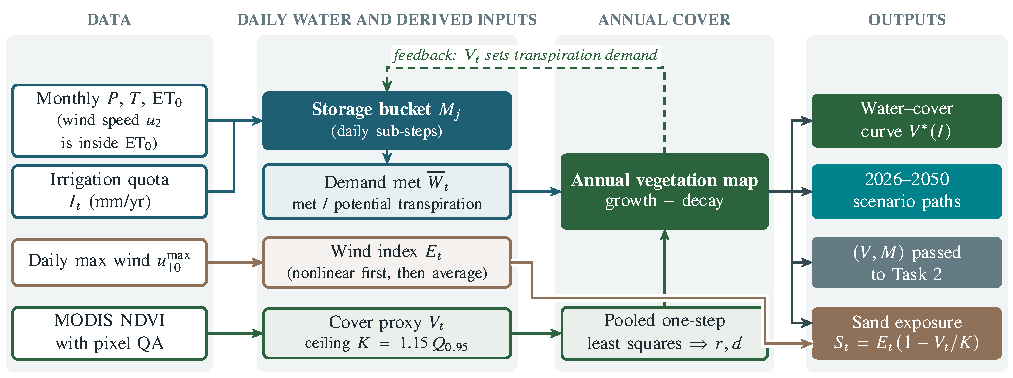
\includegraphics[width=\linewidth]{m1_structure.pdf}
  \caption{Structure of Model 1. }
  \label{fig:m1-struct}
\end{figure}

\subsection{Model construction}
\paragraph{Two states on two clocks.} The model tracks two quantities, and each one changes at its own natural speed. We picture them as two nested clocks (Figure~\ref{fig:m1-clocks}).
\begin{itemize}
  \item \textbf{Year clock (outer, slow) --- cover $V_t$ (\%).} It ticks \textbf{once per year}. Plants gain or lose cover over a season, and the satellite cover proxy is a single growing-season value, so a yearly step matches both biology and data.
  \item \textbf{Day clock (inner, fast) --- plant-available water $M_j$ (mm).} It ticks \textbf{365 times per year}. Rain and irrigation arrive in pulses and are used up within days; a yearly average would smooth away exactly the dry spells that stress plants.
\end{itemize}
\noindent The two clocks talk to each other at two points only, both at the year boundary:
\begin{itemize}
  \item \textbf{\textcircled{\scriptsize 1} Down (year $\to$ day).} At the start of each year, cover $V_t$ is \textbf{frozen} and sets each day's water demand $D_j$: a denser stand wants more water.
  \item \textbf{\textcircled{\scriptsize 2} Up (day $\to$ year).} At the end of each year, the 365 daily results are condensed into \textbf{one number}, the water-satisfaction ratio $\overline W_t$, which moves the outer ring from $V_t$ to $V_{t+1}$.
\end{itemize}
\noindent The water store $M$ is not reset: the last day of one year is the first day of the next, so wet or dry years carry over.

\begin{figure}[!htb]
  \centering
  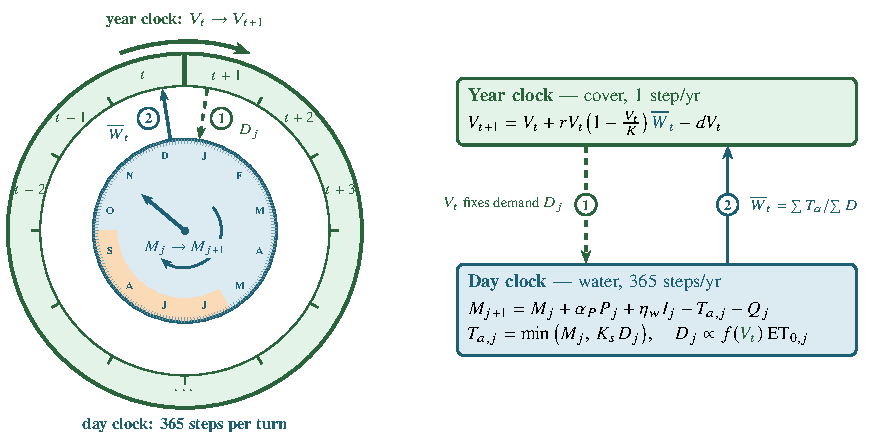
\includegraphics[width=\linewidth]{m1_two_clocks.pdf}
  \caption{The two clocks of Model 1 and their handoffs \textcircled{\scriptsize 1} and \textcircled{\scriptsize 2}.}
  \label{fig:m1-clocks}
\end{figure}

\paragraph{Cover equation: growth, decay, wind.}
\begin{equation}\label{eq:m1-veg}
V_{t+1}=V_t+\underbrace{rV_t\Big(1-\frac{V_t}{K}\Big)\overline W_t}_{\text{growth, limited by water}}
-\underbrace{dV_t}_{\text{natural decay}}
-\underbrace{kE_t\Big(1-\eta\frac{V_t}{K}\Big)V_t}_{\text{wind damage, reduced by shelter}}
\end{equation}
\emph{Growth} is logistic, stops at the local ceiling $K$, and is scaled by the water-satisfaction ratio $\overline W_t\in[0,1]$ (Eq.~\eqref{eq:m1-wbar}). \emph{Decay} removes a fixed share $d$ of cover each year. \emph{Wind damage} rises with the wind index $E_t$ (Section~\ref{sec:data}) and is reduced by the shelter factor $(1-\eta V_t/K)$ as cover thickens. Since $V=0$ stays at $0$, every scenario starts from a planted cover.

\paragraph{Water store: a daily bucket.} The root zone is treated as a bucket of capacity $C$ (Figure~\ref{fig:m1-bucket}). On each day $j$,
\begin{equation}\label{eq:m1-bucket}
\underbrace{M_{j+1}}_{\text{store tomorrow}}=\underbrace{M_j}_{\text{store today}}+\underbrace{\alpha_PP_j+\eta_wI_j}_{\text{effective inflow}}-\underbrace{T_{a,j}}_{\text{transpiration}}-\underbrace{Q_j}_{\text{overflow}},
\qquad T_{a,j}=\min\big(M,\ K_s(M)\,D_j\big).
\end{equation}
Only shares $\alpha_P$ of rain and $\eta_w$ of irrigation reach the roots, and water above capacity is lost ($Q_j$). The daily demand and the stress coefficient are
\begin{equation}\label{eq:m1-demand}
D_j=c\,\min\!\Big(1,\frac{2V_t}{V_{\mathrm{full}}}\Big)\,f(T_j)\,\mathrm{ET}_{0,j},\qquad
K_s=\min\Big\{1,\ \frac{M_j}{(1-p)C}\Big\}.
\end{equation}
The transpiration coefficient $c$ scales reference evapotranspiration $\mathrm{ET}_0$ to the demand of a full stand. Demand grows with cover until $V_t$ reaches half of the full-cover value $V_{\mathrm{full}}$, which is where cover feeds back on water, and $f(T)=\min\{1,\max\{0,(T-5)/20\}\}$ switches it on with the season. Below the stress threshold $(1-p)C$, the FAO-56 coefficient $K_s$ \cite{REF11} cuts transpiration in proportion to what is left (Figure~\ref{fig:m1-bucket}). Each daily step conserves water exactly.

\begin{figure}[!htb]
  \centering
  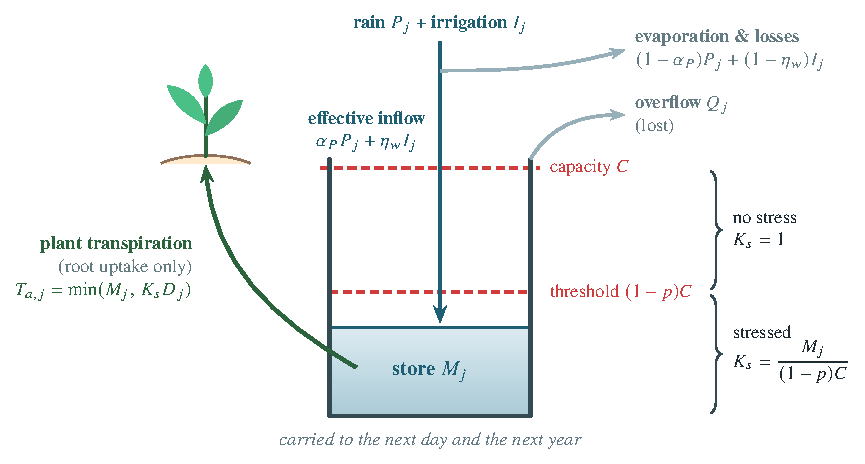
\includegraphics[width=0.95\linewidth]{m1_bucket.pdf}
  \caption{One daily step of the water bucket. $K_s$ threshold comes from reference FAO-56\cite{REF11} }
  \label{fig:m1-bucket}
\end{figure}

\paragraph{The link between the two clocks.} The daily bucket and the yearly cover update are coupled through one number, the water-satisfaction ratio
\begin{equation}\label{eq:m1-wbar}
\overline W_t=\frac{\sum_{j\in t}T_{a,j}}{\sum_{j\in t}D_j},
\end{equation}
the share of the plants' water demand actually met in year $t$. $\overline W_t=1$ means no water stress (as at the oases) and full growth rate $r$; $\overline W_t=0.4$ cuts growth to $0.4\,r$; $\overline W_t=0$ stops growth, leaving only decay and wind damage.

\subsection{Solution approach}
We fit growth and decay from data, step the coupled system through a year, and repeat the year to reach a long-run state or a scenario path.

\paragraph{Step 1: calibration by least squares.} At the seven oasis stations water is ample ($\overline W\approx1$) and wind damage is not separately identifiable, so we set $\overline W=1$ and $k=0$ there; growth and decay can then be estimated from cover alone. Fixing $K$ from each station's own record and writing $x=V/K$, Eq.~\eqref{eq:m1-veg} becomes
\begin{equation}\label{eq:m1-reg}
\underbrace{x_{s,t+1}-x_{s,t}}_{y_{s,t}:\ \text{observed change}}=r\,\underbrace{x_{s,t}(1-x_{s,t})}_{z_{1,s,t}:\ \text{growth signal}}-d\,\underbrace{x_{s,t}}_{z_{2,s,t}:\ \text{decay signal}}+\varepsilon_{s,t},
\end{equation}
where $s$ indexes stations and $\varepsilon_{s,t}$ is the one-step error. The model is linear in the unknowns $(r,d)$, so we estimate them by ordinary least squares over the set $\mathcal T$ of training pairs (target year $\le2022$, all seven stations pooled):
\begin{equation}\label{eq:m1-ls}
(\hat r,\hat d)=\arg\min_{r,d}\ \sum_{(s,t)\in\mathcal T}\big(y_{s,t}-r\,z_{1,s,t}+d\,z_{2,s,t}\big)^2 .
\end{equation}
Because the objective is quadratic in $(r,d)$, its minimiser has a closed form; Algorithm~\ref{alg:m1-ls} gives the procedure.

\begin{algorithm}[!htb]
\caption{Least-squares calibration of $r$ and $d$}\label{alg:m1-ls}
\begin{algorithmic}[1]
\Require training pairs $(x_{s,t},\,x_{s,t+1})$, $(s,t)\in\mathcal T$, with $N=|\mathcal T|$
\Ensure estimates $\hat r,\hat d$ and their bootstrap spread
\For{each pair $(s,t)\in\mathcal T$}
  \State $y_{s,t}\gets x_{s,t+1}-x_{s,t}$;\quad $z_{1,s,t}\gets x_{s,t}(1-x_{s,t})$;\quad $z_{2,s,t}\gets x_{s,t}$ \Comment{Eq.~\eqref{eq:m1-reg}}
\EndFor
\State Stack the pairs: $\bm y\in\mathbb R^{N}$ and design matrix $\bm Z=[\,\bm z_1,\ -\bm z_2\,]\in\mathbb R^{N\times2}$
\State Set the gradient of Eq.~\eqref{eq:m1-ls} to zero $\Rightarrow$ normal equations $\bm Z^\top\bm Z\,(\hat r,\hat d)^\top=\bm Z^\top\bm y$
\State Solve: $(\hat r,\hat d)^\top\gets\big(\bm Z^\top\bm Z\big)^{-1}\bm Z^\top\bm y$ \Comment{unique if columns of $\bm Z$ not proportional}
\For{$b=1,\dots,B$} \Comment{cluster bootstrap}
  \State Resample \emph{whole stations} with replacement; repeat lines 1--5 $\Rightarrow(\hat r^{(b)},\hat d^{(b)})$
\EndFor
\State Report $(\hat r,\hat d)$ with the spread of $\{(\hat r^{(b)},\hat d^{(b)})\}$
\State Check one-step error on hold-out pairs (2023--2025) against persistence $\hat x_{t+1}=x_t$
\end{algorithmic}
\end{algorithm}

\paragraph{Steps 2--3: one model year, then repeat.} Algorithm~\ref{alg:m1} shows the core loop. Repeating it under a typical climate year until $V$ and $M$ stop changing gives the long-run state for a given irrigation level. Because $\overline W$ depends on $V$, this fixed point is found numerically; we start from both a low and a high cover and accept the result only when both starts agree.

\begin{algorithm}[H]
\caption{One model year: the water store drives cover}\label{alg:m1}
\begin{algorithmic}[1]
\Require cover $V_t$, store $M$, irrigation $I_t$, one year of daily rain, ET$_0$ and temperature
\Ensure $V_{t+1}$, year-end store $M$, $\overline W_t$
\State Set daily demand $D_j$ from $V_t$ and the season \Comment{cover held fixed}
\For{each day $j$ of the year}
  \State $M\gets M+\alpha_PP_j+\eta_wI_j$;\quad spill anything above $C$ \Comment{inflow, overflow}
  \State $T_{a,j}\gets\min\big(M,K_s(M)D_j\big)$;\quad $M\gets M-T_{a,j}$ \Comment{stressed when $M$ is low}
\EndFor
\State $\overline W_t\gets\sum_jT_{a,j}/\sum_jD_j$ \Comment{Eq.~\eqref{eq:m1-wbar}}
\State $V_{t+1}\gets$ Eq.~\eqref{eq:m1-veg};\quad carry $M$ into next year
\end{algorithmic}
\end{algorithm}

\paragraph{Parameter values.} Table~\ref{tab:m1-par} lists the values used to solve the model. Only $r$ and $d$ are fitted; $K$ and $V_{\mathrm{full}}$ follow fixed rules applied to the data; the water and wind parameters cannot be fitted without field measurements, so they are stated assumptions with the ranges tested in the sensitivity analysis.

\begin{table}[H]
\centering\small
\renewcommand{\arraystretch}{1.1}
\begin{tabularx}{\linewidth}{@{}l X r c l@{}}
\toprule
Symbol & Meaning & Value & Range tested & Unit \\
\midrule
\multicolumn{5}{@{}l}{\textit{Fitted by least squares (Algorithm~\ref{alg:m1-ls})}}\\
$r$ & intrinsic growth rate & 0.547 & 0.335--1.168$^{\dagger}$ & yr$^{-1}$ \\
$d$ & natural decay rate & 0.107 & 0.077--0.202$^{\dagger}$ & yr$^{-1}$ \\
\midrule
\multicolumn{5}{@{}l}{\textit{Set from data by a fixed rule}}\\
$K$ & cover ceiling ($1.15\times$ 95th percentile of training cover) & 38.08 & -- & \% \\
$V_{\mathrm{full}}$ & cover at which demand is full (oasis end-member) & 66.59 & 64.85--69.40 & \% \\
\midrule
\multicolumn{5}{@{}l}{\textit{Assumed (no field data to fit)}}\\
$C$ & root-zone storage capacity & 75 & 30--150 & mm \\
$p$ & stress-free share of storage (FAO-56 \cite{REF11}) & 0.5 & 0.3--0.7 & -- \\
$c$ & transpiration coefficient & 1.0 & 0.7--1.2 & -- \\
$\eta_w$ & share of irrigation reaching the roots & 0.75 & 0.65--0.85 & -- \\
$\alpha_P$ & share of rain reaching the roots & 0.25 & 0--1 & -- \\
$k$ & wind-damage rate & 0 & 0--0.10 & -- \\
$\eta$ & shelter strength of dense cover & 1 & -- & -- \\
$u_T$ & wind threshold for sand drift & 5 & -- & m/s \\
$V_0$ & initial cover of a new stand & 2 & -- & \% \\
$M_0$ & initial store of a new stand & 37.5 & -- & mm \\
\bottomrule
\end{tabularx}
\caption{Model 1 parameters.}
\label{tab:m1-par}
\end{table}

\subsection{Results}
Results are for the Yutian--Minfeng section (127.95\,km $\times$ 1\,km) under a repeated 2015--2022 mean climate year; they compare water strategies, not forecasts of specific years.

\begin{figure}[!t]
  \centering
  \begin{subfigure}[t]{0.49\linewidth}
    \centering
    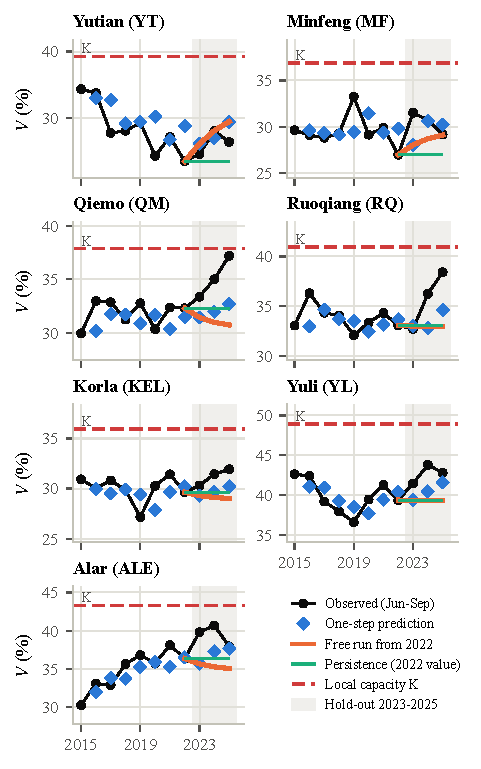
\includegraphics[width=\linewidth]{m1_f01_station_series_tall.pdf}
    \caption{Observed cover at the seven stations, 2015--2025.}
    \label{fig:m1-obs}
  \end{subfigure}\hfill
  \begin{subfigure}[t]{0.49\linewidth}
    \centering
    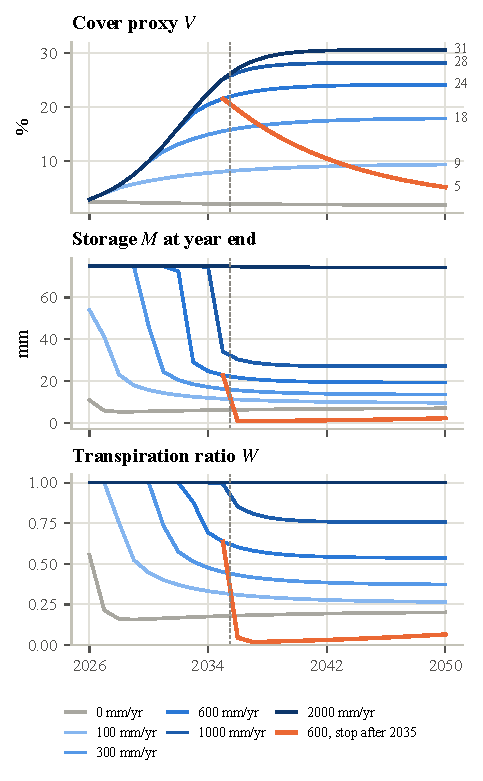
\includegraphics[width=\linewidth]{m1_f07_scenario_trajectories_tall.pdf}
    \caption{Scenario paths on the section, 2026--2050.}
    \label{fig:m1-scen}
  \end{subfigure}
  \caption{Cover and soil water over time: (a) observed, (b) modelled scenarios.}
  \label{fig:m1-paths}
\end{figure}

\paragraph{Model reliability.} An unwatered stand loses half its cover in about six years. On hold-out years the one-step forecast does not beat persistence overall (RMSE 0.064 vs 0.054 in $V/K$), but it does at Minfeng and Yutian, the two stations in our section. Figure~\ref{fig:m1-obs} shows why. Observed growing-season cover (black) varies between about 24\% and 44\% and stays below each station's ceiling $K$ (red dashed). The one-step predictions (blue) follow the level of each series but not its year-to-year spikes. In the hold-out years (grey band), cover rose sharply at Qiemo, Ruoqiang and Alar; the free run from 2022 (orange) stays near the 2022 value and misses this greening, for example 33.0\% against 38.4\% observed at Ruoqiang in 2025. At Yutian and Minfeng the free run follows the observed values more closely. Model~1 is therefore used to compare strategies, not to predict single years.
\newpage
\paragraph{Evolution of the state variables.} From a planted cover of 2\%, cover and soil water pass through three phases (Figure~\ref{fig:m1-scen}):
\begin{enumerate}\setlength{\itemsep}{1pt}\setlength{\parsep}{0pt}
  \item \textbf{Establishment: growth, not water, limits cover.} Young plants use little water, so with 300\,mm/yr or more the store stays full ($\overline W=1$) and the surplus drains. All such quotas give the same 9.9\% cover by 2030, so water above about 300\,mm/yr is wasted in this phase.
  \item \textbf{Transition: cover drains the store.} Demand rises with cover until it exceeds supply. The store then drops from capacity within about two years and settles slowly (to about 13\,mm at 300\,mm/yr), and $\overline W$ falls below one. This is the feedback at work: more cover means less water per plant, which slows growth.
  \item \textbf{Plateau (after 15--25 years): both settle.} Each quota gives its own steady cover and store, e.g.\ 17.9\% and 13\,mm at 300\,mm/yr, or 24.1\% and 19\,mm at 600\,mm/yr.
\end{enumerate}
The plateau lasts only while water is supplied. If irrigation stops after ten years, the store empties within a year, $\overline W$ falls to 0.03--0.07, and cover drops from 21.5\% to 12.7\% in five years and to 5.1\% in fifteen.

\paragraph{Controlling factors: water supply.} Water supply is the main control. Rain alone (52\,mm/yr against about 1,700\,mm/yr of evaporative demand) holds only 1.8\% cover.

\noindent\begin{minipage}[t]{0.585\linewidth}
\vspace{0pt}
Irrigation raises long-run cover quickly at first, then with strongly diminishing returns (Figure~\ref{fig:m1-curve}a):
\begin{enumerate}\setlength{\itemsep}{1pt}\setlength{\parsep}{0pt}
  \item the first 100\,mm/yr adds 7.7 percentage points;
  \item going from 500 to 600\,mm/yr adds only 1.6;
  \item above about 1,500\,mm/yr, cover stops at a ceiling of 30.6\%.
\end{enumerate}
The bucket explains this shape: at 300\,mm/yr only 37\% of demand is met (Figure~\ref{fig:m1-curve}b), so the deficit, not the ceiling $K$, keeps cover at 18\%; above 1,500\,mm/yr extra water only overflows.
\end{minipage}\hfill
\begin{minipage}[t]{0.395\linewidth}
\vspace{0pt}\centering
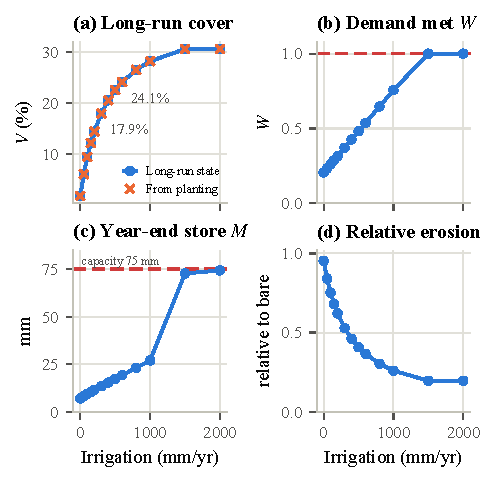
\includegraphics[width=\linewidth]{m1_f06_water_cover_curve_half.pdf}
\captionof{figure}{Long-run state against irrigation. Red dashed lines are limits.}
\label{fig:m1-curve}
\end{minipage}

\noindent\begin{minipage}[t]{0.615\linewidth}
\vspace{0pt}
\paragraph{Controlling factors: demand, delivery and wind.} With water supply fixed, we varied the other factors one at a time (Figure~\ref{fig:m1-sens}). They fall into three groups:
\begin{enumerate}\setlength{\itemsep}{1pt}\setlength{\parsep}{0pt}
  \item \textbf{Factors that shift long-run cover by 1--3 points:} the transpiration coefficient $c$ ($-1.7$ to $+3.4$ points at 300\,mm/yr), irrigation efficiency ($\pm1.2$) and the effective rain fraction ($-0.5$ to $+1.4$). All three act through $\overline W$, the supply-to-demand ratio.
  \item \textbf{Factors that change soil water but not long-run cover:} storage capacity and the stress threshold. Without overflow, all inflow is eventually transpired, so $\overline W$ depends only on inflow and demand; these factors change only the storage level and its timing.
  \item \textbf{Wind damage, the largest uncertainty.} The data cannot pin down its rate, so it is a scenario; at the highest rate tested it cuts cover at 300\,mm/yr by 24\% (17.9\% to 13.6\%), more than any water parameter.
\end{enumerate}

\paragraph{Summary.} Cover and soil water rise together, settle at a level set by the water supply, and decline once water stops. Water supply is the main control, with sharply diminishing returns; demand, delivery efficiency and wind damage shift the result.
\end{minipage}\hfill
\begin{minipage}[t]{0.365\linewidth}
\vspace{0pt}\centering
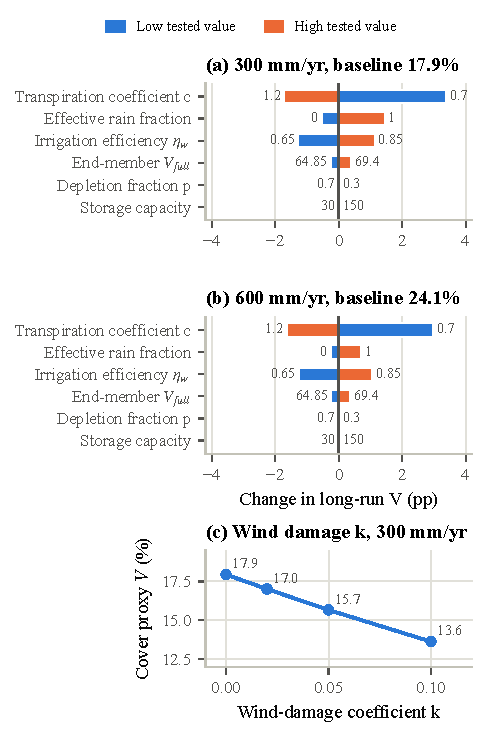
\includegraphics[width=\linewidth]{m1_f09_sensitivity_tall.pdf}
\captionof{figure}{Sensitivity of long-run cover to one-at-a-time changes and to wind damage.}
\label{fig:m1-sens}
\end{minipage}
